\textbf{Ejemplo 3}\\
\vspace{2mm}

Una persona tiene dos deudas una de  250.000 COP pagadera en 3 meses y otra de 400.000  COP pagadera en 7 meses. Si desea cambiar la forma de cancelarlas mediante dos pagos iguales de X COP cada uno con vencimiento en 5 meses y 12 meses respectivamente, determinar el valor de los pagos suponiendo una tasa del 24\% (namv) nominal anual mes vencido.\\ \\
%\newpage %USAR SOLO SI EL SOLUCIÓN QUEDA SOLO Y ES NECESARIO BAJARLO A LA SIGUIENTE PAGINA
\textbf{Solución.}\\
%La tabla ira centrada
\begin{center}
 \renewcommand{\arraystretch}{1.5}% Margenes de las celdas
 %Creación de la cuadricula de 3 columnas
 \begin{longtable}[H]{|p{0.5\linewidth}|p{0.5\linewidth}|}
  \hline
  \multicolumn{2}{|c|}{\cellcolor[HTML]{FFB183}\textbf{1. Declaración de variables}}                          \\ \hline
  Deuda Inicial      & Deuda equivalente                                                                      \\
  $D_1= 250.000 COP $ & $n_1 = 5 pmv$                                                                          \\
  $n_1=3 pmv$        & $n_2 = 10 pmv$                                                                         \\
  $D_2= 400.000 COP $ & $j = 24 \% namv$                                                                     \\
  $n_2=7 pmv$        & $i = 2 \% pmv$                                                                        \\ \hline
  \multicolumn{2}{|c|}{\cellcolor[HTML]{FFB183}\textbf{2. Tabla de flujo de caja}}                            \\ \hline
  \multicolumn{2}{|p{\columnwidth}|}{
  \begin{center}
   \begin{tabular}{|p{4cm}|p{4cm}|p{4cm}|}
    \hline
    \textbf{Periodo} & \textbf{Deuda Inicial} & \textbf{Deuda Equivalente} \\ \hline

    0                &  COP                      &  COP                          \\ \hline
    1                &  COP                      &  COP                          \\ \hline
    2                &  COP                      &  COP                          \\ \hline
    3                &  250.000 COP              &  COP                          \\ \hline
    4                &  COP                      &  COP                          \\ \hline
    5                &  COP                      &  X COP                        \\ \hline
    6                &  COP                      &  COP                          \\ \hline
    7                &  400.000 COP              &  COP                          \\ \hline
    8                &  COP                      &  COP                          \\ \hline
    9                &  COP                      &  COP                          \\ \hline
    10               &  COP                      &  COP                          \\ \hline
    11               &  COP                      &  COP                          \\ \hline
    12               &  COP                      &  X COP                        \\ \hline
   \end{tabular}
  \end{center}
  }                                                                                                           \\ \hline
  \multicolumn{2}{|c|}{\cellcolor[HTML]{FFB183}\textbf{3. Fórmulas utilizadas}}                               \\ \hline
  \multicolumn{2}{|l|}{Mediante el uso de Excel:}                                                             \\
  \multicolumn{2}{|l|}{VNA (Valor neto actual): Devuelve el valor neto presente de una inversión}                      \\ \hline
  \multicolumn{2}{|c|}{\cellcolor[HTML]{FFB183}\textbf{4. Desarrollo en Excel}}                               \\ \hline
  \multicolumn{2}{|l|}{Se aplicará la función VNA de la siguiente forma:}                                      \\
  \multicolumn{2}{|c|}{ 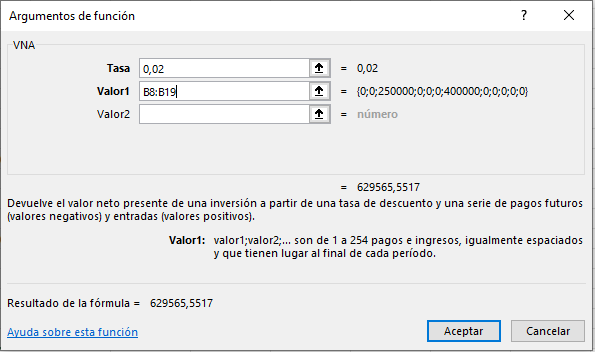
\includegraphics[trim=-5 -5 -5 -5 ,width=1\columnwidth]{3/Ejem3.PNG}}                 \\
  \multicolumn{2}{|p{\columnwidth}|}{
  Esta función se aplicará de la siguiente forma en las dos celdas donde se desee obtener
  el Valor presente de las deudas originales y de las deudas equivalentes.\newline

  = -VNA(0,02;B7:B19) = -=VNA(0,02;C7:C19)\newline

  Luego se aplicará la formula Función Objetivo de la siguiente forma:
  }                                                                                                           \\
  \multicolumn{2}{|c|}{ 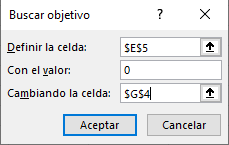
\includegraphics[trim=-5 -5 -5 -5 ,width=0.5\columnwidth]{3/Ejem3.2.PNG}} \\ \hline
  \multicolumn{2}{|c|}{\cellcolor[HTML]{FFB183}\textbf{5. Respuesta}}                                         \\ \hline
  \multicolumn{2}{|p{\columnwidth}|}{
  \begin{center}
   \begin{tabular}{|p{4cm}|p{4cm}|p{4cm}|}
    \hline
    \textbf{Periodo} & \textbf{Deuda Inicial} & \textbf{Deuda Equivalente} \\ \hline


    0                &  COP                      &  COP                          \\ \hline
    1                &  COP                      &  COP                          \\ \hline
    2                &  COP                      &  COP                          \\ \hline
    3                &  25.000,00 COP             &  COP                          \\ \hline
    4                &  COP                       &  COP                          \\ \hline
    5                &  COP                      &  35.424,00 COP                 \\ \hline
    6                &  COP                      &  COP                          \\ \hline
    7                &  40.000,00 COP            &  COP                          \\ \hline
    8                &  COP                      &  COP                          \\ \hline
    9                &  COP                      &  COP                          \\ \hline
    10               &  COP                      &  COP                          \\ \hline
    11               &  COP                      &  COP                          \\ \hline
    12               &  COP                      &  35.424,00 COP                 \\ \hline
   \end{tabular}
  \end{center}

  Debe realizar dos pagos con el valor de 35.423,66 COP cada uno.
  }                                                                                                           \\ \hline
  \multicolumn{2}{|c|}{\cellcolor[HTML]{FFB183}\textbf{6. Gráfica}}                                           \\ \hline
  \multicolumn{2}{|c|}{No es necesaria la realización de una gráfica para este ejercicio.}                    \\ \hline
 \end{longtable}
 %\newline \newline %USARLO SI CREES QUE ES NECESARIO
\end{center}
